\chapter{Power Series}

Consider the function $f(x) = \frac{1}{1-x}$. This looks similar to the value 
of convergent geometric series, $\sum_{n=1}^\infty ar^{n-1} = \frac{a}{1-r}$. 
If we let $a = 1$ and $r = x$, then we see that $\sum_{n=1}^\infty x^{n-1} = 
\frac{1}{1-x}$. We can reindex to begin at $n=0$ and see that:
$$\frac{1}{1-x} = \sum_{n=0}^\infty x^n$$

This is a \textbf{power series}. \index{power series}We use power series in place of functions for many 
applications, such as integrals where an explicit antiderivative don't exist, solving 
differential equations, and computer scientists representing functions on 
computers. Consider $f(x) = \frac{1}{1-x^2}$. What is $\int 
f(x)\,dx$? We can't directly use u-substitution, and this is not a derivative of 
any inverse trigonometric function. [You may have realized we could integrate 
this explicitly by using partial fractions, but this is not true for other 
functions, and we are using this as a demonstration anyway.] One way to 
evaluate this integral would be to represent $f(x)$ as a power series, then 
integrate the series. This is easier, since we know how to take the integral 
of any polynomial ($\int x^n\,dx = \frac{1}{n+1}x^{n+1} + C$). First, we 
discuss what power series are further.

\section{Power Series}
Power series are series of the form
$$\sum_{n=0}^\infty c_n x^n = c_0 + c_1 x + c_2 x^2 + c_3 x^3 + \cdots + c_n 
x^n$$

for some fixed $x$. Depending on $x$, the series may converge or diverge. For 
example, the power series $\sum_{n=0}^\infty x^n$ converges for $ -1 < x < 1$ 
and diverges for all other values of $x$. This is because $\sum_{n=0}^\infty 
x^n$ is essentially a geometric series with $r = x$, which we already know 
converges for $|r|<1$. 

The form given above is for a power series centered on $0$, but a power series 
can be centered on any value, $a$. In that case, it looks like this:
$$\sum_{n=0}^\infty c_n (x - a)^n = c_0 + c_1(x - a) + c_2(x - a)^2 + \cdots + 
c_n(x - a)^n$$

Which we say is a \textit{power series in }$(x - a)$, or a \textit{power 
series centered at }$a$, or a \textit{power series about }$a$. 

\textbf{Example}: Find a power series representation for $f(x) = \frac{2x - 4}{
x^2 - 4x +3}$. 

\textbf{Solution}: Since we know $\frac{1}{1-x} = \sum_{n=0}^\infty x^n$, we 
will use partial fractions to decompose the function into two fractions. (The 
process is left as an exercise for the student.) We find that:
$$\frac{2x - 4}{x^2 - 4x + 3} = \frac{1}{x - 1} + \frac{1}{x-3}$$
Noting that $\frac{1}{x-1} = (-1) \cdot\frac{1}{1-x}$, we can say that:
$$\frac{1}{x-1} = (-1) \cdot \sum_{n=0}^\infty x^n$$
Now, let's look at $\frac{1}{x-3}$. We can show that:
$$\frac{1}{x-3} = \frac{\frac{1}{3}}{\frac{x}{3}-1} = \frac{1}{3} \frac{1}{
\frac{x}{3}-1} = \frac{-1}{3} \frac{1}{1-\frac{x}{3}}$$
Substituting $\frac{x}{3}$ for $x$ into $\frac{1}{1-x} = \sum_{n=0}^\infty 
x^n$ we see that:
$$\frac{1}{1-\frac{x}{3}} = \sum_{n=0}^\infty \left(\frac{x}{3} \right)^n$$
Therefore:
$$\frac{1}{x-3} = \left( \frac{-1}{3} \right) \sum_{n=0}^\infty \left( 
\frac{x}{3} \right)^n$$
Adding the terms, we see that:
$$\frac{1}{x-1} + \frac{1}{x-3} = (-1) \sum_{n=0}^\infty x^n + \left( 
\frac{-1}{3} \right) \sum_{n=0}^\infty \left( \frac{x}{3} \right)^n$$

\section{Power Series Convergence}
Sometimes, you will be asked to find one or more values of $x$ 
for which a power series converges. To do this, choose a test to apply, 
then find $x$ such that the test is passed. 

\textbf{Example}: For what values of $x$ is the series $\sum_{n=0}^\infty n!x^n$ 
convergent?

\textbf{Solution}: We will apply the Ratio Test (since there is a factorial in 
the series) and find $x$ such that $\lim_{n \to \infty} \left| \frac{a_{n+1}}{
a_n} \right| < 1$. 
$$\lim_{n \to \infty} \left| \frac{a_{n + 1}}{a_n} \right| = \lim_{n \to 
\infty} \left| \frac{(n+1)!x^{n+1}}{n!x^n} \right|$$
$$= \lim_{n \to \infty} \frac{(n+1) n! x \cdot x^n}{n!x^n} = \lim_{n \to 
\infty} \frac{(n+1) \cdot x}{1}$$
which converges to $0$ when $x=0$ and diverges for all other values of $x$. 
Therefore, $\sum_{n=0}^\infty n!x^n$ converges if $x=0$. 

\textbf{Example}: For what values of $x$ does the series $\sum_{n=1}^\infty 
\frac{(x-4)^n}{2n}$ converge?

\textbf{Solution}: We will use the Ratio Test again. We are looking for an $x$ 
such that:
$$\lim_{n \to \infty} \left| \frac{a_{n+1}}{a_n} \right| < 1$$
$$\lim_{n \to \infty} \left| \frac{\frac{(x-4)^{n+1}}{2(n+1)}}{\frac{(x-4)^n}{
2n}} \right| < 1$$
$$\lim_{n \to \infty} \left| \frac{(x-4)(x-4)^n}{2n + 2} \cdot \frac{2n}{(x-4)^
n} \right| < 1$$
$$\lim_{n \to \infty} \left| \frac{(x-4)(x-4)^n(2n)}{(x-4)^n(2n+2)} \right| < 
1$$
$$\lim_{n \to \infty} \left| \frac{(x-4)(2n)}{2n + 2} \right| < 1$$
$$\lim_{n \to \infty} \left| \frac{2(x-4)}{2 + \frac{2}{n}} \right| < 1$$
$$2 \cdot \lim_{n \to \infty} \left| \frac{x-4}{1+ \frac{1}{n}} \right| < 1$$
$$2 \cdot \left| x-4 \right| < 1$$
$$\left| x-4 \right| < \frac{1}{2}$$\\
Which is true when 
$$-\frac{1}{2} < x-4 < \frac{1}{2}$$
$$3.5 < x < 4.5$$

We are not done yet, though! We know the series converges for $3.5 < x < 4.5$ 
and diverges for $x < 3.5$ and $x > 4.5$. What about when $x = 3.5$ and $x = 
4.5$? (These are the cases where the Ratio Test is indeterminate, because 
$\lim_{n \to \infty} \left| \frac{a_{n+1}}{a_n} \right| = 1$.) We need to test 
each case. Substituting $x = 3.5$ into the series yields:
$$\sum_{n=1}^\infty \frac{(3.5-4)^n}{2n} = \sum_{n=1}^\infty \frac{\left( 
\frac{-1}{2} \right)^n}{2n}$$
$$= \sum_{n=1}^\infty \frac{(-1)^n}{n \cdot 2^{n+1}}$$
This is an alternating series, so we apply the alternating series test. First, 
we check that $|a_{n+1}| < |a_n|$:
$$\frac{1}{(n+1) \cdot 2^{n+2}}  < \frac{1}{n \cdot 2^{n+1}}$$
Which is true for all $n > 0$. Next, we check if $\lim_{n \to \infty} |a_n| = 0$:
$$\lim_{n \to \infty} \frac{1}{n \cdot 2^{n+1}} = \frac{1}{\infty} = 0$$
Therefore, $\sum_{n=1}^\infty \frac{(-1)^n}{n \cdot 2^{n+1}}$ is convergent 
and $\sum_{n=1}^\infty \frac{(x-4)^n}{2n}$ is convergent for $x = 3.5$. Next, we 
test $x=4.5$ for convergence:
$$\sum_{n=1}^\infty \frac{(4.5-4)^n}{2n} = \sum_{n=1}^\infty \left( 
\frac{1}{2} \right)^n \cdot \frac{1}{2n} = \sum_{n=1}^\infty \left( 
\frac{1}{2} \right)^{n+1} \frac{1}{n}$$
This series is less than the harmonic series $\sum_{n=1}^\infty \frac{1}{n}$ 
for all $n$. We know the harmonic series diverges, therefore, by the direct 
comparison test, $\sum_{n=1}^\infty \left( \frac{1}{2} \right)^{n+1} 
\frac{1}{n}$ must also diverge. So, our final answer to the original question 
is that the series is convergent fort $3.5 \leq x < 4.5$. 

\subsection{Radius of Convergence}
There are three possible outcomes when testing a power series $\sum_{n=0}^
\infty c_n (x-a)^n$ for convergence:
\begin{enumerate}
\item The series only converges for $x = a$
\item The series converges for all $x$
\item The series converges if $|x - a| < R$ and diverges for $|x - a| > R$, 
where $R$ is some positive number
\end{enumerate}

We call $R$ the \textbf{radius of convergence} \index{radius of convergence}. 
If we rearrange $|x - a| < R$, we can see why this is called a radius (see 
figure \ref{fig:radiusofconv}): 
$$a - R < x < a + R$$

\begin{figure}[htbp]
\centering
    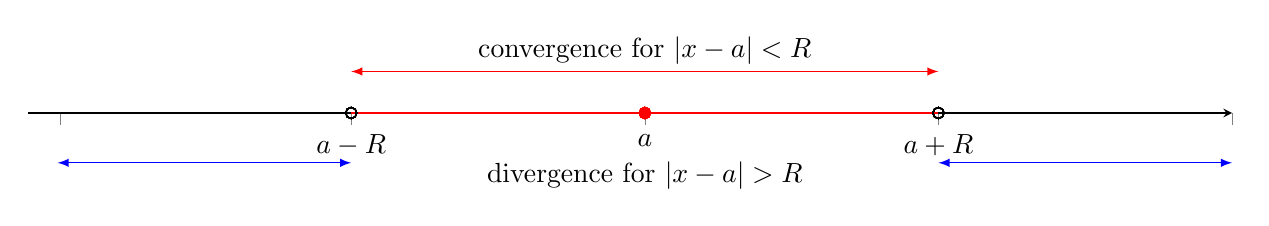
\begin{tikzpicture}
        \begin{axis}[axis y line = none, width = 2*\axisdefaultwidth, 
        height = 0.25*\axisdefaultwidth, axis lines = center, 
        xtick align = outside, xmin = -0.1, xmax = 4, 
        xtick = {0.01, 1, 2, 3, 4}, xticklabels = {, $a - R$, $a$, 
        $a + R$, }, ymin = -0.5, ymax = 0.5, 
        clip = false]
        \addplot[mark=o, black](1, 0);
        \addplot[mark=o, black](3, 0);
        \draw[red, thick] (1, 0) -- (3, 0);
        \addplot[mark=*, red] (2, 0);
        \node[] at (2, 1.5) {convergence for $|x - a| < R$};
        \draw[latex-latex, red] (1, 1) -- (3, 1);
        \node[] at (2, -1.5) {divergence for $|x - a| > R$};
        \draw[latex-latex, blue] (0, -1.2) -- (1, -1.2);
        \draw[latex-latex, blue] (3, -1.2) --(4, -1.2);
        \end{axis}
    \end{tikzpicture}
    \caption{$R$ is called the radius of convergence because it is half the 
    width of the window of convergence}
    \label{fig:radiusofconv}
\end{figure}

When $x = a \pm R$, the series could be convergent or divergent. You will need 
to test the endpoints of the windown of convergence to determine if the 
interval is open or closed. Thus, there are four possiblities for the interval 
of convergence:
\index{interval of convergence}
\begin{enumerate}
\item $(a - R, a + R)$
\item$[a - R, a + R)$
\item$(a - R, a + R]$
\item$[a - R, a + r]$
\end{enumerate}

It is important to check each endpoint to determine the interval of convergence individually. 

In the example of $\sum_{n=1}^\infty \frac{(x-4)^n}{2n}$ (shown above), 
$a = 4$ and $R = 0.5$, and we found that the power series is convergent for 
$x \in [3.5, 4.5)$. 

\textbf{Example}: For what values of $x$ is the Bessel function $J_0 (x) = 
\sum_{n=0}^\infty \frac{(-1)^n x^{2n}}{2^{2n}(n!)^2}$ convergent? 

\textbf{Solution}: Because there is a factorial, we will apply the Ratio Test:
$$\lim_{n \to \infty} \left| \frac{a_{n + 1}}{a_n} \right| <  1$$
$$\lim_{n \to \infty} \left| \frac{\frac{(-1)^{n + 1} x^{2(n + 1)}}{2^{2(n + 1
)}((n + 1)!)^2}}{frac{(-1)^n x^{2n}}{2^{2n}(n!)^2}} \right| < 1$$
$$\lim_{n \to \infty} \frac{x^{2n} x^2 2^{2n} n! n!}{2^{2n} 2^2 (n = 1)! (n + 
1)! x^{2n}} < 1$$
$$\lim_{n \to \infty} \frac{x^2 n! n!}{2^2 (n + 1)n! (n + 1)n!} < 1$$
$$\lim_{n \to \infty} \frac{x^2}{4(n + 1)^2} = 0 < 1$$
Because $lim_{n \to \infty} \left| \frac{a_{n + 1}}{a_n} \right| = 0$ for all 
$x$, the Bessel function $J_0 (x) = \sum_{n=0}^\infty \frac{(-1)^n x^{2n}}{2^{
2n}(n!)^2}$ is convergent for all real values of $x$, and the interval of 
convergence is $(-\infty, \infty)$. 

\textbf{Example}: Find the radius and interval of convergence for the series 
$\sum_{n=0}^\infty \frac{(-3)^n x^n}{\sqrt{n + 1}}$.

\textbf{Solution}: Again, we apply the ratio test to find values of $x$ such 
that $\lim_{n \to \infty} \left| \frac{a_{n + 1}}{a_n} \right| < 1$:
$$\lim_{n \to \infty} \left| \frac{(-3)^{n + 1} x^{n + 1}}{\sqrt{n + 1 + 1}} 
\cdot \frac{\sqrt{n + 1}}{(-3)^n x^n} \right| < 1$$
$$\lim_{n \to \infty} \left| \frac{(-3) x}{\sqrt{n + 2}} \cdot \frac{\sqrt{n + 
1}}{1} \right| < 1$$
$$\lim_{n \to \infty} \left| (-3)x \sqrt{\frac{n + 2}{n + 1}} \right| < 1$$
$$3|x| \lim_{n \to \infty} \sqrt{\frac{n + 2}{n + 1}} < 1$$
$$3|x| \lim_{n \to \infty} \sqrt{\frac{1 + 2/n}{1 + 1/n}} = 3|x|(1) < 1$$
$$3|x| < 1$$
$$|x| < \frac{1}{3}$$

Therefore, the radius of convergence is $\frac{1}{3}$. We need to test the 
endpoints, $x = \frac{-1}{3}$ and $x = \frac{1}{3}$, to determine the interval 
of convergence. First, we will test if $\sum_{n=0}^\infty \frac{(-3)^n x^n}{
\sqrt{n + 1}}$ when $x = \frac{-1}{3}$:
$$\sum_{n=0}^\infty \frac{(-3)^n \left( \frac{-1}{3} \right)^n}{\sqrt{n + 1}} 
= \sum_{n = 0}^\infty \frac{1^n}{\sqrt{n + 1}} = \sum_{n = 0}^\infty \frac{1}{
\sqrt{n + 1}}$$
This is a $p$-series such that $ p < 1$, so it is divergent, and our original 
series does not converge for $x = \frac{-1}{3}$. Next, we test $x = \frac{1}{3}$:
$$\sum_{n=0}^\infty \frac{(-3)^n \left( \frac{1}{3} \right)^n}{\sqrt{n + 1}} = 
\sum_{n = 0}^\infty \frac{(-1)^n}{\sqrt{n + 1}}$$
which is an alternating series that converges by the alternating series test. 
Therefore, the interval of convergence for $\sum_{n=0}^\infty \frac{(-3)^n x^n}
{\sqrt{n + 1}}$ is $x \in \left( \frac{-1}{3}, \frac{1}{3} \right]$. 

\begin{Exercise}[label = radconv1]
[This problem was originally presented as a no-calculator, multiple-choice 
question on the 2012 AP Calculus BC exam.] What is the radius of convergence 
of the series $\sum_{n=0}^\infty \frac{(x - 4)^{2n}}{3^n}$?
\end{Exercise}

\begin{Answer}[ref = radconv1]
Since this sum has terms to the $n^{th}$ power, we will apply the Root Test, 
which states a series is convergent if $\lim_{n \to \infty} \sqrt[n]{\left| 
a_n \right|} < 1$. 
$$\lim_{n \to \infty} \sqrt[n]{\left| \frac{(x - 4)^{2n}}{3^n} \right|} < 1$$
$$\lim_{n \to \infty} \left| \frac{(x - 4) ^ {2n/n}}{3^{n/n}} \right| < 1$$
$$\lim_{n \to \infty} \frac{\left| (x-4)^2 \right|}{3} < 1$$
$$(x - 4)^2 < 3$$
$$\left| x - 4 \right| < \sqrt{3}$$
Therefore, the radius of convergence is $\sqrt{3}$. 
\end{Answer}

\begin{Exercise}[label = radconv2]
[This problem was originally presented as a no-calculator, multiple-choice 
question on the 2012 AP Calculus BC exam.] A power series is given by 
$\frac{x}{3} - \frac{x^3}{5} + \frac{x^5}{7} - \frac{x^7}{9} + \cdots$. Write 
the series in sigma notation and use the Ratio Test to determine the interval 
of convergence.
\end{Exercise}

\begin{Answer}[ref = radconv2]
We see that the series is alternating, so we know it involves $(-1)^n$ (we 
will begin indexing at $n = 0$). The powers of $x$ are given by $x^{2n+1}$ and 
the denominators are given by $2n + 3$. Therefore, the sum in sigma notation 
is $\sum_{n=0}^\infty (-1)^n \frac{x^{2n+1}}{2n+3}$. Applying the ratio test, 
the series is convergent when:
$$\lim_{n \to \infty} \left| \frac{(-1)^{n+1} x^{2(n+1)+1}}{2(n+1)+3} \frac{2n+
3}{(-1)^n x^{2n+1}} \right| < 1$$
$$\lim_{n \to \infty} \left| \frac{x^{2n+3}}{2n+5} \frac{2n+3}{x^{2n+1}} 
\right| < 1$$
$$\left| x^2 \right| \lim_{n \to \infty} \frac{2n+3}{2n+5} < 1$$
$$\left| x^2 \right| < 1$$
$$\left| x \right| < 1$$
So, we know that the series is convergent on the open interval $x \in (-1, 1)$. 
We check the endpoints, $x = -1, 1$ for convergence. 
$$\sum_{n=0}^\infty \frac{(-1)^n (-1)^{2n+1}}{2n+3} = \sum_{n=0}^\infty \frac{
(-1)^{3n+1}}{2n+3}$$
When $x = -1$, the series is an alternating series such that $\left| a_{n+1} 
\right| < \left|a_n \right|$ and $\lim_{n \to \infty} a_n = 0$. Therefore, the 
series converges for $x = -1$.
$$\sum_{n=1}^\infty (-1)^n \frac{(1)^{2n+1}}{2n+3} = \sum_{n=1}^\infty \frac{
(-1)^n}{2n+3}$$
which is also an alternating series such that $\left| a_{n+1} \right| < \left| 
a_n \right|$ and $\lim_{n \to \infty} a_n = 0$. Therefore, the series 
converges for $x = 1$ and the interval of convergence is $x \in [-1, 1]$, 
which can also be written as $-1 \leq x \leq 1$. 
\end{Answer}

\section{Calculus with Power Series}
\index{power series!calculus with}
You can integrate and differentiate power series. Let $f(x) = \sum_{n=0}^\infty 
c_n (x-a)^n$. Recall that $f(x)$ is just a very long polynomial and that the 
derivative of a polynomial $x^n$ is $n \cdot x^{n-1}$. We can then state that:
$$\frac{d}{dx}f(x) = \frac{d}{dx} \left[c_0 + c_1(x-a)^1 + c_2(x-a)^2 + \cdots 
+ c_n(x-a)^n \right]$$
$$f'(x) = 0 + c_1 + 2c_2(x-a)^1 + \cdots + n c_n(x-a)^{n-1}$$
$$f'(x) = \sum_{n=1}^\infty c_n(x-a)^{n-1}$$

which is true when $x$ is in the interval of convergence for the series. 

Similarly, we know $\int x^n\,dx = \frac{1}{n+1}x^{n+1}$. We can then say that:
$$\int f(x) \,dx = \int \left[c_0 + c_1(x-a)^1 + c_2(x-a)^2 + \cdots + c_n(x-a)
^n\right],dx$$
$$\int f(x)\,dx = C + c_0(x-a) + \frac{c_1}{2}(x-a)^2 + \frac{c_2}{3}(x-a)^3 + 
\cdots \frac{c_n}{n+1}(x-a)^{n+1}$$
$$\int f(x)\,dx = C + \sum_{n=0}^\infty \frac{c_n}{n+1}(x-a)^{n+1}$$

Where $C$ is the integration constant. Again, this is true when $x$ is in the 
interval of convergence for the series. 

\textbf{Example}: Express $\frac{1}{(1-x)^2}$ as a power series by 
differentiating $\frac{1}{1-x}$. 

\textbf{Solution}: Recall that $\frac{1}{1-x} = \sum_{n=0}^\infty x^n$ when 
$|x|<1$. 
$$\frac{1}{1-x} = \sum_{n=1}^\infty x^n$$
Differentiating both sides:
$$\frac{d}{dx} \left[ \frac{1}{1-x} \right] = \frac{d}{dx} \sum_{n=0}^\infty 
x^n$$
$$(-1) \cdot \frac{1}{(1-x)^2} \cdot \frac{d}{dx}(1-x) = \sum_{n=1}^\infty 
nx^{n-1}$$
$$\frac{1}{(1-x)^2} = \sum_{n=1}^\infty nx^{n-1}$$
Reindexing to begin at $n = 0$
$$\frac{1}{(1-x)^2} = \sum_{n=0}^\infty (n+1)x^n$$
Because $\sum_{n=0}^\infty$ has a radius of convergence of 1, so does $\sum_{
n=0}^\infty (n+1)x^n$. We can confirm our series makes sense by plotting the 
partials sums for $n = 3, 5, and 7$ with the original function (see figure 
\ref{power1}).

\begin{figure}[htbp]
\centering
    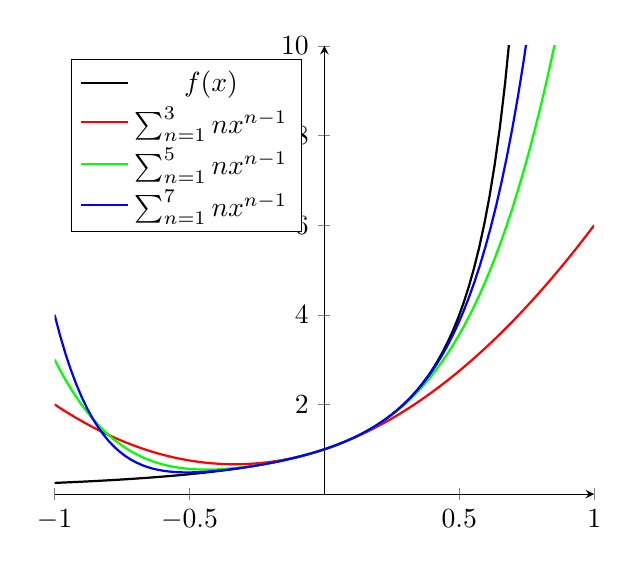
\begin{tikzpicture}
	\begin{axis}[xmin = -1, xmax = 1, axis lines = center, ymin = 0, ymax = 10, 
	legend pos = north west]
            \addplot[black, thick, domain = -1:0.9, samples = 100]{1/(1-x)^2};
            \addlegendentry{$f(x)$};
            \addplot[red, thick, domain = -1:1, samples = 100]{1 + 2*x + 3*x^2};
            \addlegendentry{$\sum_{n=1}^3 nx^{n-1}$};
            \addplot[green, thick, domain = -1:1, samples = 100]{1 + 2*x + 
            3*x^2 + 4*x^3 + 5*x^4};
            \addlegendentry{$\sum_{n=1}^5 nx^{n-1}$};
            \addplot[blue, thick, domain = -1:1, samples = 100]{1 + 2*x + 
            3*x^2 + 4*x^3 + 5*x^4 + 6*x^5 + 7*x^6};
            \addlegendentry{$\sum_{n=1}^7 nx^{n-1}$};
        \end{axis}
    \end{tikzpicture}
    \caption{The function $f(x) = \frac{1}{(1-x)^2}$ is equal to the power 
    series $\sum_{n=1}^\infty nx^{n-1}$}
    \label{power1}
\end{figure}

\textbf{Example}: Find a power series representing $\ln{(1+x)}$. 

\textbf{Solution}: We know that $\frac{d}{dx} \frac{1}{1-x} = \ln{(1-x)}$. 
Replacing $x$ with $-x$, we see that:
$$\frac{1}{1-(-x)} = \frac{1}{1+x} = \sum_{n=0}^\infty (-x)^n$$
which converges for $|x| < 1$. We can then integrate both sides:
$$\int \frac{1}{1+x}\,dx = \int \left[ \sum_{n=0}^\infty (-x)^n \right] \,dx$$
$$\ln{(1 + x)} = \int \left( 1 - x + x^2 - x^3 + \cdots \right)\,dx $$
$$\ln{(1 + x)} = C + x - \frac{x^2}{2} + \frac{x^3}{3} + \cdots + (-1)^{n-1} \frac{x^n}{n}$$
$$\ln{(1 + x)} = \sum_{n=1}^\infty (-1)^{n-1} \frac{x^n}{n} + C$$
when $|x|<1$. To find $C$, substitute $x = 0$ and solve:
$$\ln{(1 + 0)} = C + \sum_{n=1}^\infty (-1)^{n-1} \frac{0^n}{n} = C + 0$$
$$C = \ln{1} = 0$$
So, our final answer is $\ln{(1 + x)} = \sum_{n=1}^\infty (-1)^{n-1} \frac{x^n}{
n}$. 

\begin{Exercise}[label = seriescalc1]
Find a power series representation for $f(x) = \arctan{x}$. 
\end{Exercise}

\begin{Answer}[ref = seriescalc1]
Recall that $\frac{d}{dx} \arctan{x} = \frac{1}{1+x^2}$. Replacing $x$ with 
$-x^2$, we see that $\frac{1}{1 + x^2} = \frac{1}{1- (-x^2)} = \sum_{n=0}^
\infty \left[ -x^2 \right]^n = \sum_{n=0}^\infty (-1)^n x^{2n}$. Then we can 
also say that $\arctan{x} = \int \frac{1}{1 + x^2}\,dx = \int \left[ sum_{n=0}
^\infty (-1)^n x^{2n} \right]\,dx$. Evaluating the integral, $\int \left[ sum_
{n=0}^\infty (-1)^n x^{2n} \right]\,dx = \sum_{n=0}^\infty (-1)^n \int 
x^{2n}\,dx = C + \sum_{n=0}^\infty \frac{(-1)^n x^{2n+1}}{2n+1}$. Knowing that 
$\arctan{0} = 0$, we find that $C = 0$ and $\arctan{x} = \sum_{n=0}^\infty 
\frac{(-1)^n x^{2n+1}}{2n+1}$. 
\end{Answer}